\documentclass[12pt,letterpaper, onecolumn]{exam}
\usepackage{amsmath}
\usepackage{amssymb}
\usepackage{sidecap}
\usepackage{tabularx}
\usepackage{csquotes}
\usepackage{makecell}
\usepackage{hyperref}
\hypersetup{
    colorlinks=true,
    linkcolor=blue,
    filecolor=magenta,      
    urlcolor=black,
    pdftitle={Overleaf Example},
    pdfpagemode=FullScreen,
}
%\usepackage[left=0.5cm,right=0.5cm,top=0.5cm,bottom=0.5cm]{geometry}
\usepackage[usestackEOL]{stackengine}
%\setstacktabbedgap{1ex} 
\usepackage{tikz}
\usetikzlibrary{decorations.pathreplacing}
\usetikzlibrary{fadings}
\def\layersep{2.5cm}

\usepackage{enumitem}
\usepackage{algorithm}
\usepackage{algpseudocode}

%\usepackage[shortlabels]{enumitem}
%\usepackage{enumerate}
\usepackage[lmargin=71pt, tmargin=0.8in]{geometry}  %For centering solution box

% \chead{\hline} % Un-comment to draw line below header
\thispagestyle{empty}   %For removing header/footer from page 1

\usepackage{listings}
\usepackage{xcolor}

\definecolor{codegreen}{rgb}{0,0.6,0}
\definecolor{codegray}{rgb}{0.5,0.5,0.5}
\definecolor{codepurple}{rgb}{0.58,0,0.82}
\definecolor{backcolour}{rgb}{0.95,0.95,0.92}

\lstdefinestyle{mystyle}{
    backgroundcolor=\color{backcolour},   
    commentstyle=\color{codegreen},
    keywordstyle=\color{magenta},
    numberstyle=\tiny\color{codegray},
    stringstyle=\color{codepurple},
    basicstyle=\ttfamily\footnotesize,
    breakatwhitespace=false,         
    breaklines=true,                 
    captionpos=b,                    
    keepspaces=true,                 
    numbers=left,                    
    numbersep=5pt,                  
    showspaces=false,                
    showstringspaces=false,
    showtabs=false,                  
    tabsize=2
}

\lstset{style=mystyle}




\begin{document}



\newtheorem{theorem}{Theorem}[section]
\newtheorem{problem}{Problem}
\newtheorem{proposition}{Proposition}[section]
\newtheorem{lemma}{Lemma}[section]
\newtheorem{corollary}[theorem]{Corollary}
\newtheorem{example}{Example}[section]
\newtheorem{definition}[problem]{Definition}

\newcommand{\BEQA}{\begin{eqnarray}}
\newcommand{\EEQA}{\end{eqnarray}}
\newcommand{\define}{\stackrel{\triangle}{=}}
\bibliographystyle{IEEEtran}
\raggedbottom
\setlength{\parindent}{0pt}
\providecommand{\mbf}{\mathbf}
\providecommand{\norm}[1]{\lVert#1\rVert}
\providecommand{\pr}[1]{\ensuremath{\Pr\left(#1\right)}}
\providecommand{\qfunc}[1]{\ensuremath{Q\left(#1\right)}}
\providecommand{\sbrak}[1]{\ensuremath{{}\left[#1\right]}}
\providecommand{\lsbrak}[1]{\ensuremath{{}\left[#1\right.}}
\providecommand{\rsbrak}[1]{\ensuremath{{}\left.#1\right]}}
\providecommand{\brak}[1]{\ensuremath{\left(#1\right)}}
\providecommand{\lbrak}[1]{\ensuremath{\left(#1\right.}}
\providecommand{\rbrak}[1]{\ensuremath{\left.#1\right)}}
\providecommand{\cbrak}[1]{\ensuremath{\left\{#1\right\}}}
\providecommand{\lcbrak}[1]{\ensuremath{\left\{#1\right.}}
\providecommand{\rcbrak}[1]{\ensuremath{\left.#1\right\}}}
\let\vec\mathbf

\newlist{mydesc}{description}{1} % create a new list called mydesc, of type "description"
\setlist[mydesc]{
  align=left, % use the align-format defined above
  leftmargin=0pt, % indentation for all the lines
  labelindent=1em, % horizontal space before label
  labelsep=0pt
   % horizontal space after label -- set to zero because we add space via "leftwithbar"
}



\begingroup  
    \centering
    
    \LARGE Weekly Report 3 - t-SNE\\[0.5em]
    
    \large Ganji Varshitha\par
    \large AI20BTECH11009\par
\endgroup
\rule{\textwidth}{0.4pt}
\pointsdroppedatright   %Self-explanatory
\printanswers
\newcommand\Solution{
  \textbf{Solution:}\\}
\newcommand{\myvec}[1]{\ensuremath{\begin{bmatrix}#1\end{bmatrix}}}
 %Replace "Ans:" with starting keyword in solution box

 \subsection*{Introduction}
t-Distributed Stochastic Neighbor Embedding (t-SNE) is a technique for dimensionality reduction that is particularly well suited for the visualization of high-dimensional datasets.\\
This is a part of manifold learning also known as non-linear dimensionality reduction.\\ The algorithm was developed by Laurens van der Maaten and Geoffrey Hilton.

\subsection*{Algorithm}
\begin{figure}[!h]
\centering
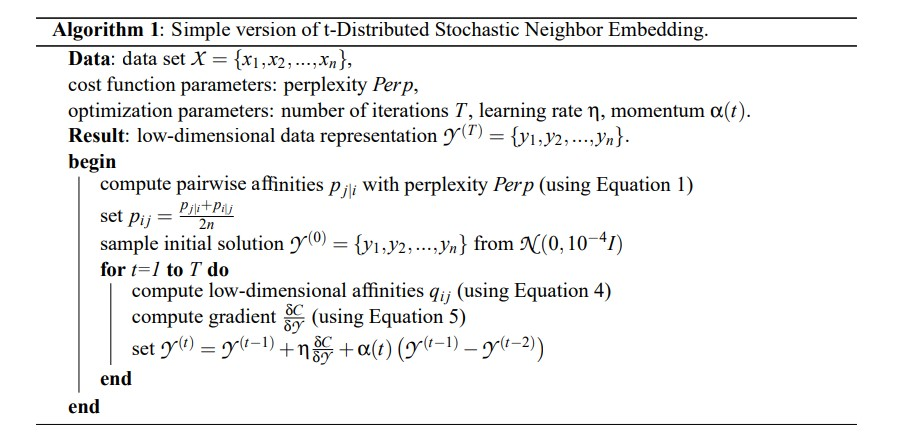
\includegraphics[width = \textwidth]{../images/tsne_alg}
\end{figure}

In contrast to reduce the high-dimensional dataset to low-dimensional data, we refer the low-dimensional data representation $\mathcal{Y}$ as a bijective map, and to the low-dimensional representations yi of individual datapoints as map points.\\
We try to achieve the same structure of high-dimensional data in the low-dimensional map i.e the points which are closer to a point are placed near that point in low dimensional space also.\\
The algorithm has 2 stages:
\begin{enumerate}
\item Convert distances to probabilities that data point x$_i$ will choose data point x$_j$ as its neighbour.
\\ Conditional probability between two points is given by
\begin{align}
p_{j|i} ={}& \frac{\exp\left(-\left|| x_i – x_j\right||^2 \big/ 2\sigma_i^2\right)}{\displaystyle\sum_{k \neq i} \exp\left(-\left|| x_i – x_k\right||^2 \big/ 2\sigma_i^2\right)}
\end{align}
For t-SNE, we use symmetric SNE, i.e
\begin{align}
p_{ij} = {}& \frac{p_{j|i} + p_{i|j}}{2N} \;  \; \text{where N is number of datapoints}
\end{align}
\item We need to evaluate the map from $\mathcal{X} \rightarrow \mathcal{Y}$
\begin{itemize}
\item We can compute conditional probability for map points using t-Student distribution with one degree of freedom.
\begin{align}
q_ij = {}& \frac{(1+ ||y_i - y_j||^2)^{-1}}{\sum_{k} \sum_{k \neq l} (1+ ||y_k - y_l||^2)^{-1}}
\end{align}
\item Since we want both the probabilities to be very close to each other, we minimise the kullback - Leiber divergence between the two distributions
\begin{align}
KL(P||Q) ={}& \sum_{i, j} p_{ij} \, \log \frac{p_{ij}}{q_{ij}}.
\end{align}
We achieve this using gradient descent stated in the algorithm above.
\end{itemize}
\end{enumerate}






\end{document}